\section{Architettura}
L'obiettivo principale del progetto è la creazione di un servizio captcha insieme a un'applicazione web 
dimostrativa che ne faccia uso, al fine di illustrarne il funzionamento. Per raggiungere questo obiettivo, 
il prodotto è stato realizzato come un'API REST.

La componente centrale dell'applicazione risiede nel back-end, dove è stato utilizzato il framework Laravel 
per la codifica.

La parte back-end è responsabile principalmente della gestione delle richieste della generazione e della verifica del servizio captcha. 
D'altro canto, per la parte front-end, è stata creata una semplice pagina HTML che utilizza JavaScript per fare 
richieste all'API REST. Questa pagina fornisce un'interfaccia utente elementare attraverso la quale gli utenti possono 
interagire con il servizio captcha.

\subsection{Diagrammi delle classi}

Il diagramma delle classi si può suddividere in varie sezioni, le quali svolgono ognuna una parte portante del progetto. Le sezioni sono:
\begin{itemize}
    \item Generazione del Captcha;
    \item Captcha Resource;
    \item Verifica del Captcha;
    \item Gestione delle chiavi per l'encrypt e decrypt delle soluzioni del captcha;
    \item Download e elaborazione delle immagini.
\end{itemize}

Per lo sviluppo delle varie funzionalità elencate il gruppo ha sfruttato diversi strumenti forniti dal framework Laravel, 
come gli eloquent Model che forniscono un metodo semplice ed intuitivo per interagire con le entità presenti nel DB, e delle classi 
Controller per poter gestire la logica di gestione delle richieste nel modo più chiaro possibile. Infatti i Controllers possono 
raggruppare la logica di gestione delle richieste correlate in una singola classe.

\subsubsection{Generazione del Captcha}

\begin{figure}[H]
    \centering
    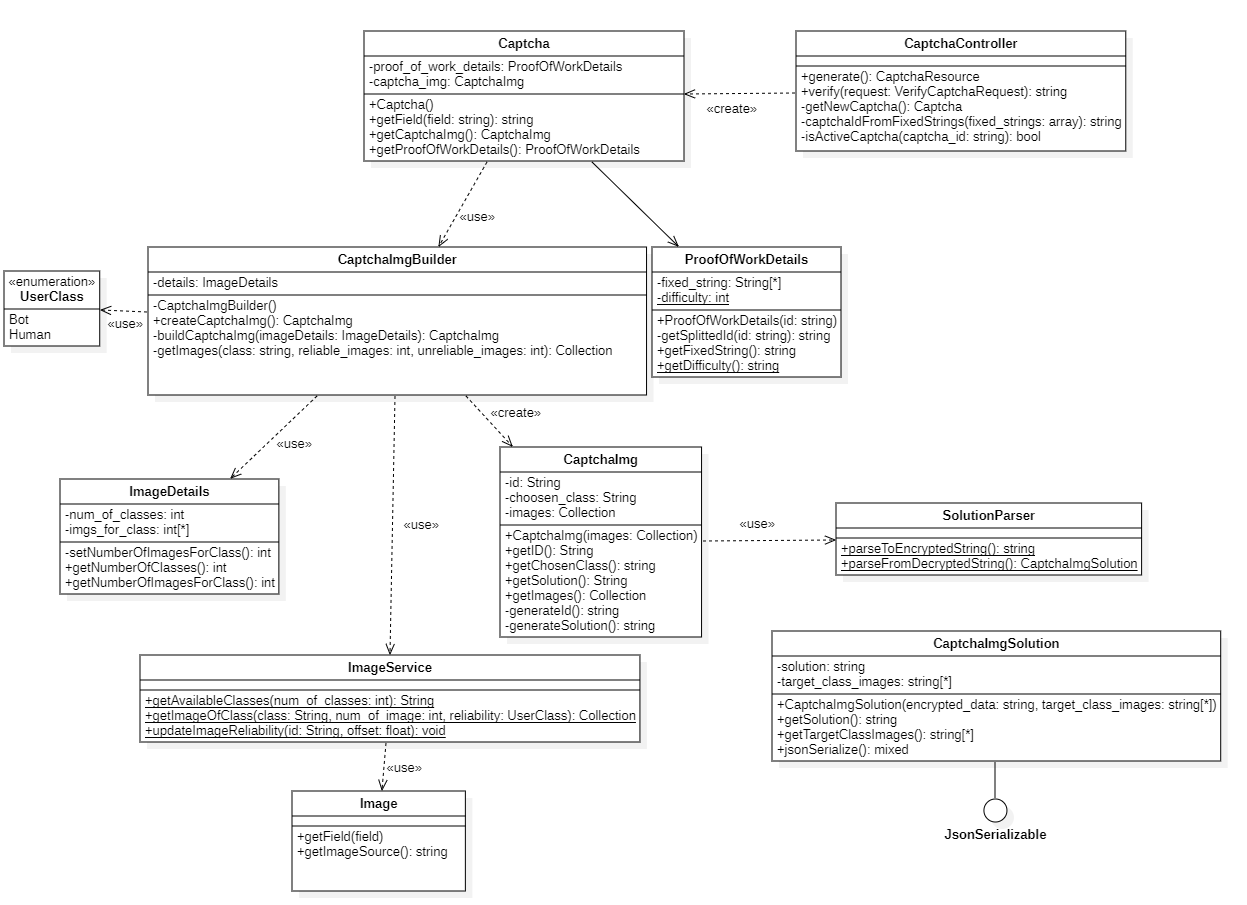
\includegraphics[scale = 0.45]{img/generate.png}\\
    \caption{Diagramma delle classi. Generazione del Captcha}
\end{figure}
\newpage

Nella figura sopra viene mostrata la logica utilizzata per la generazione di un  Captcha.
\begin{itemize}
    \item  Ogni Captcha è composto da:
    \begin{itemize}
        \item 9 immagini in bianco e nero con solo i contorni visibili;
        \item L'immagine honeypot, invisibile all'utente;
        \item Il proof of work.
    \end{itemize}
\end{itemize}

In particolare:
\begin{itemize}
    \item \textbf{CaptchaController}: Classe cardine del progetto, la quale si occupa di gestire tutte le richieste che verranno fatte alla route dell'API. In questa classe è anche contenuto il metodo che ritornerà l'oggetto CaptchaResource a seguito di una richiesta da parte dell'utente;
    \item \textbf{Captcha}: Classe che si occupa di mettere insieme tutti i pezzi che compongono il Captcha, ovvero immagini, honeypot e proof of work. Questa classe viene creata dal Controller quando viene richiesto un Captcha;
    \item \textbf{CaptchaImgBuilder}: Classe singleton che si occupa dell'effettiva creazione della parte del Captcha che contiene le immagini e l'honeypot. Fa inoltre utilizzo di una enumerazione per la gestione dell'affidabilità delle immagini;
    \item \textbf{ProofOfWorkDetails}: Classe che contiene i dati necessari per il calcolo dei nonce nel proof of work;
    \item \textbf{ImageDetails}: Classe che contiene i dettagli utili alla creazione delle 9 immagini che comporranno il Captcha, quali il numero di classi e di immagini per classe che dovrà avere. Viene utilizzata dalla classe CaptchaImgBuilder;
    \item \textbf{CaptchaImg}: Classe che contiene le varie informazioni che la parte del captcha composta dalle immagini deve avere. È l'oggetto che la classe CaptchaImgBuilder va a creare;
    \item \textbf{ImageService}: Classe che contiene i metodi per le chiamate al DB riguardanti il Model delle immagini. Viene dalla classe CaptchaImgBuilder per recuperare le immagini da inserire nel Captcha;
    \item \textbf{Image}: Eloquent Model che contiene le informazioni dell'oggetto immagine. Viene utilizzato da ImageService;
    \item \textbf{Solution Parser}: Classe che gestisce l'encrypting della soluzione, che è in formato json, così che l'utente non possa decifrarla;
    \item \textbf{CaptchaImgSolution}: Classe che contiene le informazioni della soluzione della parte del Captcha composta dalle immagini.
\end{itemize}

\subsubsection{Captcha Resource}
\begin{figure}[H]
	\centering
	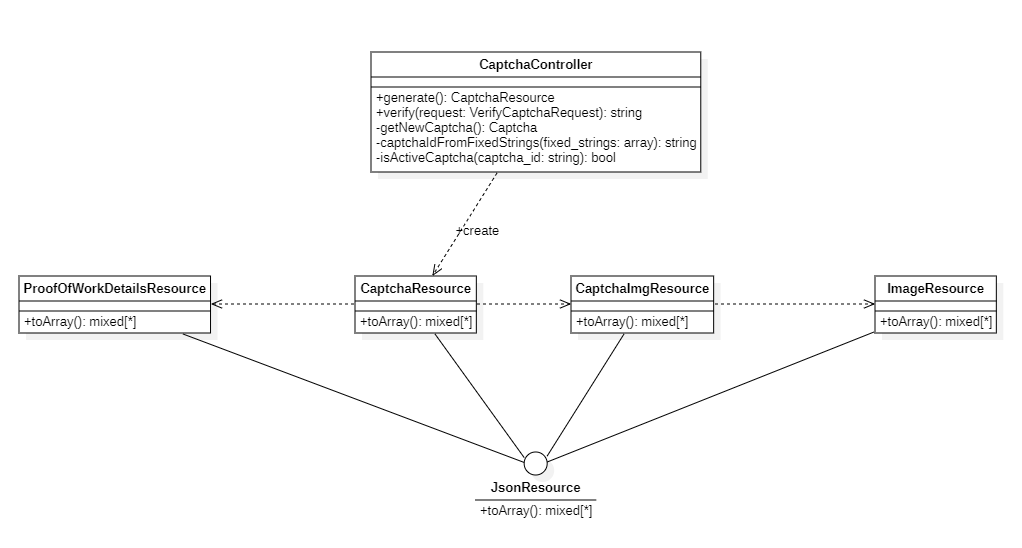
\includegraphics[scale = 0.6]{img/captcha_resource.png}\\
	\caption{Diagramma delle classi. Captcha resource}
\end{figure}

Nella figura sopra viene mostrata la logica utilizzata per la gestione delle informazioni che si vogliono passare all'utente al seguito di una richiesta. Infatti dopo la creazione di un captcha, viene creato dal Controller l'oggetto CaptchaResource, il quale sarà un json che contiene solamente le informazioni chiave per il caricamento del captcha lato front-end e la soluzione criptata che servirà durante la verifica del Captcha.

In particolare:
\begin{itemize}
	\item \textbf{CaptchaController}: Dopo aver creato il Captcha, genera l'oggetto CaptchaResource il quale contiene le varie informazioni da passare in risposta alla richiesta dell'utente;
	\item \textbf{CaptchaResource}: Classe Eloquent Resource che utilizza le classi CaptchaImgResource e ProofOfWorkDetailsResource per generare il json che verrà poi inviato all'utente;
	\item \textbf{CaptchaImgResource}: Classe Eloquent Resource che seleziona le informazioni da inviare all'utente per la parte del Captcha immagini. Utilizza la classe ImageResource per le informazioni delle immagini contenute nel Captcha;
	\item \textbf{ProofOfWorkDetailsResource}: Classe Eloquent Resource che seleziona le informazioni da inviare all'utente per la parte del proof of work;
	\item \textbf{ImageResource}: Classe Eloquent Resource che seleziona le informazioni che ogni immagine dovrà avere nella risposta all'utente.
\end{itemize}
\newpage

\subsubsection{Verifica del Captcha}

\begin{figure}[H]
	\centering
	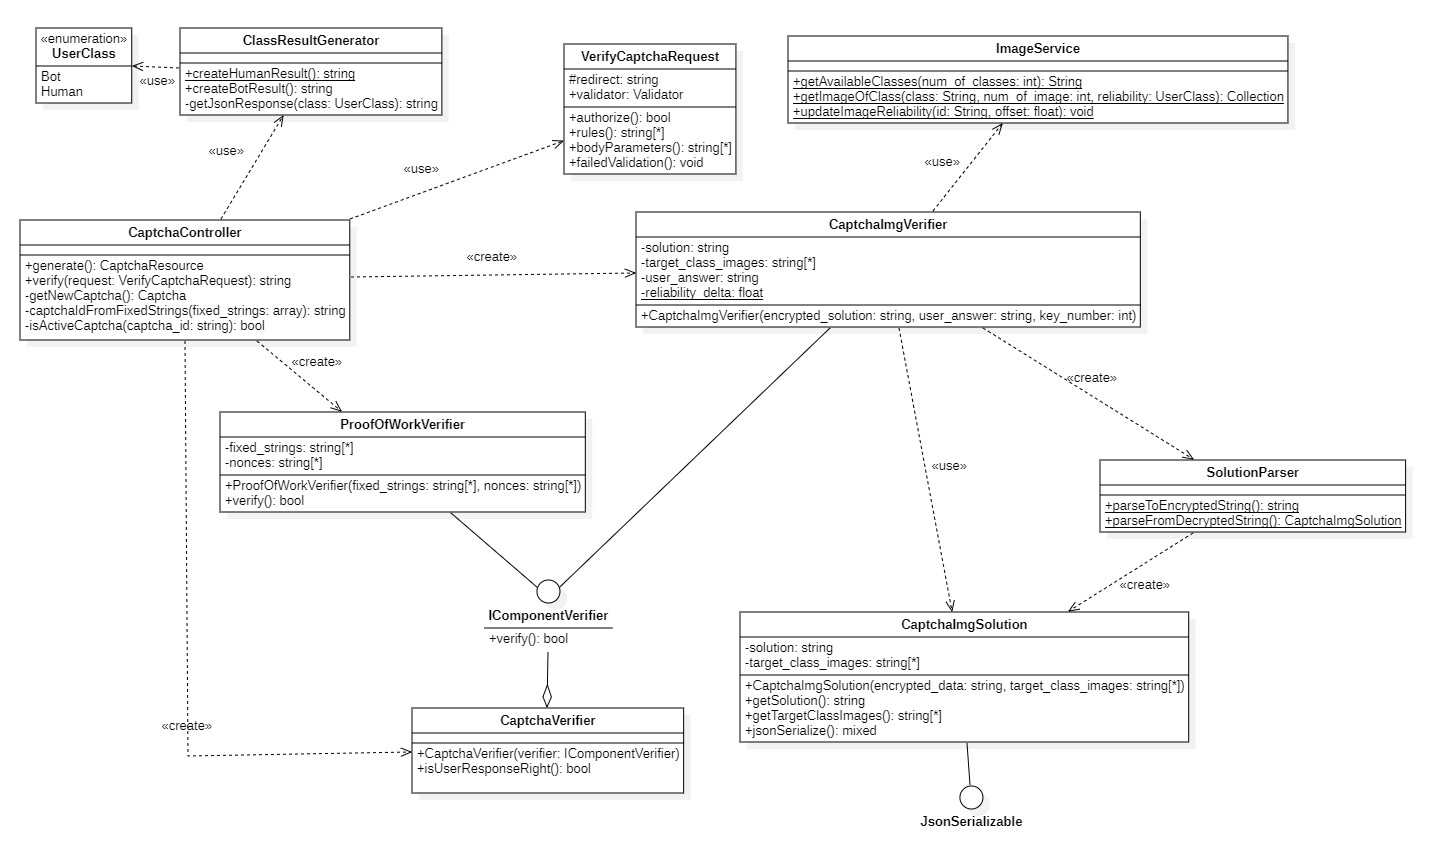
\includegraphics[scale = 0.45]{img/verify.png}\\
	\caption{Diagramma delle classi. Verifica del Captcha}
\end{figure}

Nella figura sopra viene mostrata la logica utilizzata per la verifica dei Captcha inviati dagli utenti. Come punto centrale c'è sempre il CaptchaController che gestisce tutte le richieste. Quest'ultimo andrà a creare i vari verificatori che controlleranno se l'utente ha dato una risposta valida o no. Viene poi generato un json che verrà criptato e inviato come risposta.
In particolare:
\begin{itemize}
	\item \textbf{CaptchaController}: Questa classe si occupa anche di gestire le richieste per la verifica di un Captcha, andando prima a validare se la risposta inviata coerente a quella aspettata e poi andando a creare i verificatori che andranno a controllare la correttezza effettiva del Captcha;
	\item \textbf{VerifyCaptchaRequest}: Classe che controlla se la risposta inviata dall'utente è nel formato richiesto;
	\item \textbf{CaptchaVerifier}: Questa classe utilizza i verificatori CaptchaImgVerifier e ProofOfWorkVerifier per controllare se la risposta dell'utente è corretta o meno;
	\item \textbf{IComponentVerifier}: Questa classe possiede il metodo verify che verrà implementato dai due verificatori; 
	\item \textbf{CaptchaImgVerifier}: Classe che verifica la correttezza della soluzione dell'utente per la parte del Captcha composto dalle immagini, andando inoltre ad utilizzare la classe ImageService per aggiornare l'affidabilità delle immagini nel DB;
	\item \textbf{ProofOfWorkVerifier}: Classe che verifica la correttezza dei nonce calcolati dall'utente durante il proof of work;
	\item \textbf{SolutionParser}: Classe utilizzata da CaptchaImgVerifier per decriptare la soluzione corretta del Captcha inviata alla'utente;
	\item \textbf{CaptchaImgSolution}: Classe che contiene gli attributi della soluzione del Captcha. Creata da SolutionParser per fornire la soluzione decriptata a CaptchaImgVerifier;
	\item \textbf{ImageService}: Classe utilizzata dal CaptchaImgVerifier per aggiornare l'affidabilità delle immagini all'interno del DB;
	\item \textbf{ClassResultGenerator}: Classe che genera il json criptato che sarà dato in risposta alla soluzione inviata dall'utente. Questo json contiene il risultato dell'operazione di verifica.
\end{itemize}

\newpage

\subsubsection{Gestione delle chiavi e dell'encrypting}

\begin{figure}[H]
	\centering
	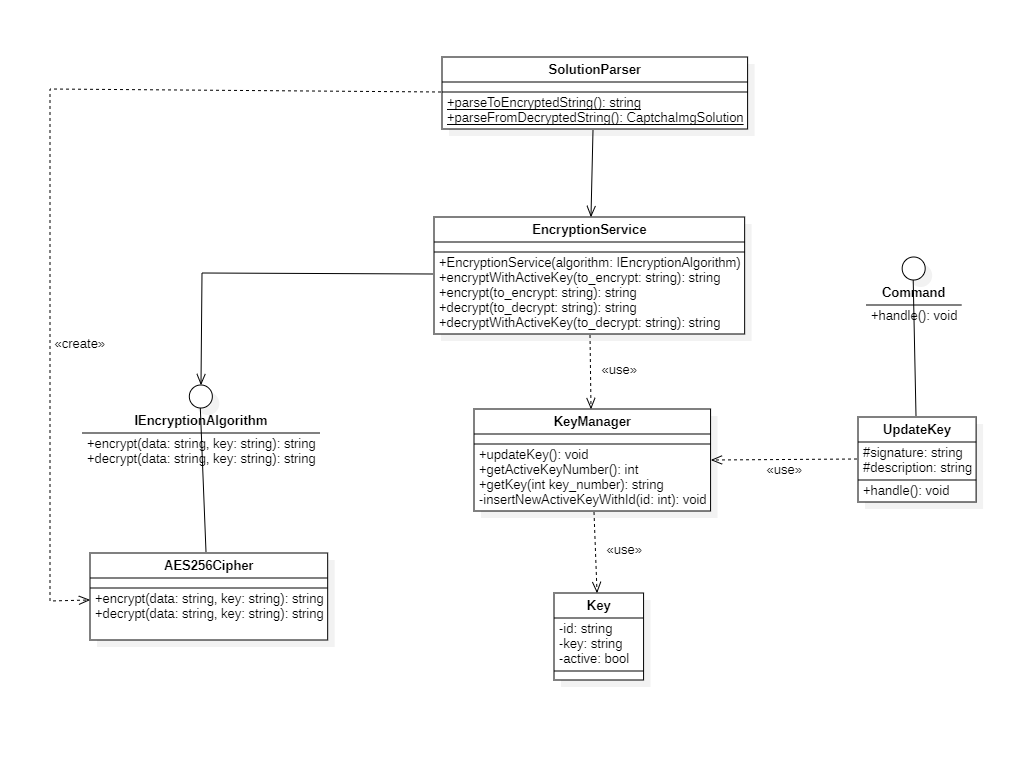
\includegraphics[scale = 0.55]{img/key_manager.png}\\
	\caption{Diagramma delle classi. Gestione delle chiavi e dell'encrypting}
\end{figure}
\newpage

\subsubsection{Download e elaborazione delle immagini}

\begin{figure}[H]
    \centering
    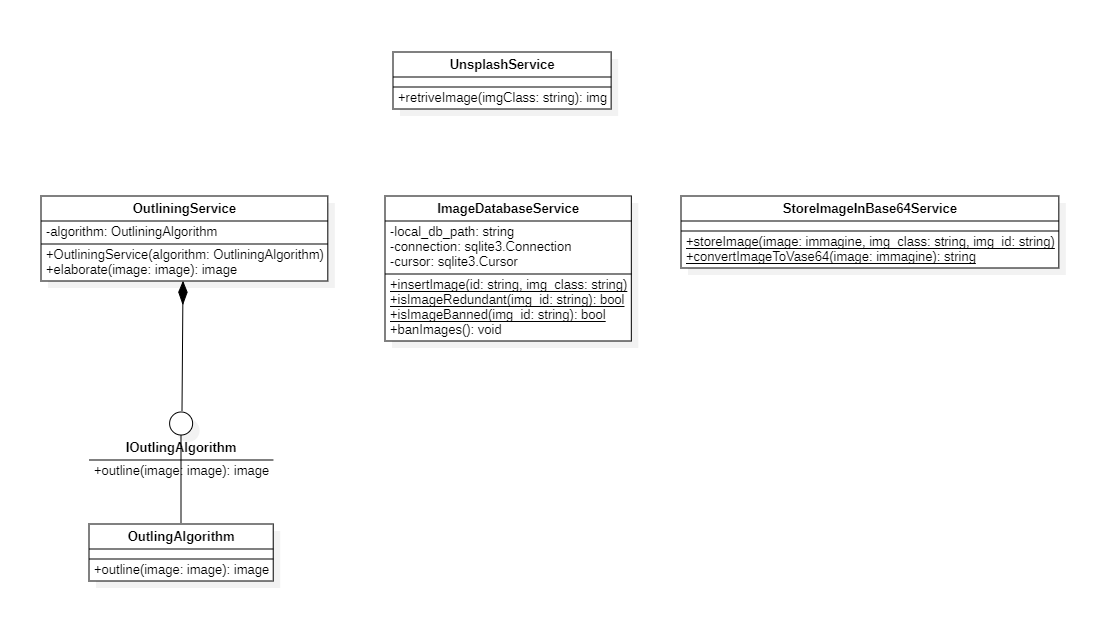
\includegraphics[scale = 0.6]{img/downloadImg.png}\\
    \caption{Diagramma delle classi. Recupero delle immagini da Unsplash}
\end{figure}

La figura sopra riportata rappresenta il metodo di download delle immagini dal sito di Unsplash, la rielaborazione di tali immagini e il metodo di salvataggio. Vengono eseguiti con il seguente ordine:
\begin{enumerate}
    \item Viene scaricato l'immagine di una determina classe;
    \item Rielaborazione dell'immagine eliminando i colori e tenendo solo il contorno.
    \item Conversione dell'immagine in base64;
    \item Salvataggio dell'immagine del database.
\end{enumerate}

In particolare:
\begin{itemize}
    \item \textbf{UnsplashService}: download dell'immagine;
    \item \textbf{OutliningService}: elaborazione dell'immagine;
    \item \textbf{OutilningAlgorithm}: algoritmo di elaborazione dell'immagine;
    \item \textbf{StoreImageInBase64Service}: salvataggio dell'immagine in formato base64 usando come path \textit{classe/id immagine};
    \item \textbf{ImageDatabaseService}: salvataggio dell'immagine nel database.
\end{itemize}

\subsection{Architettura di dettaglio}

\subsubsection{Strategy pattern}

\begin{figure}[H]
    \centering
    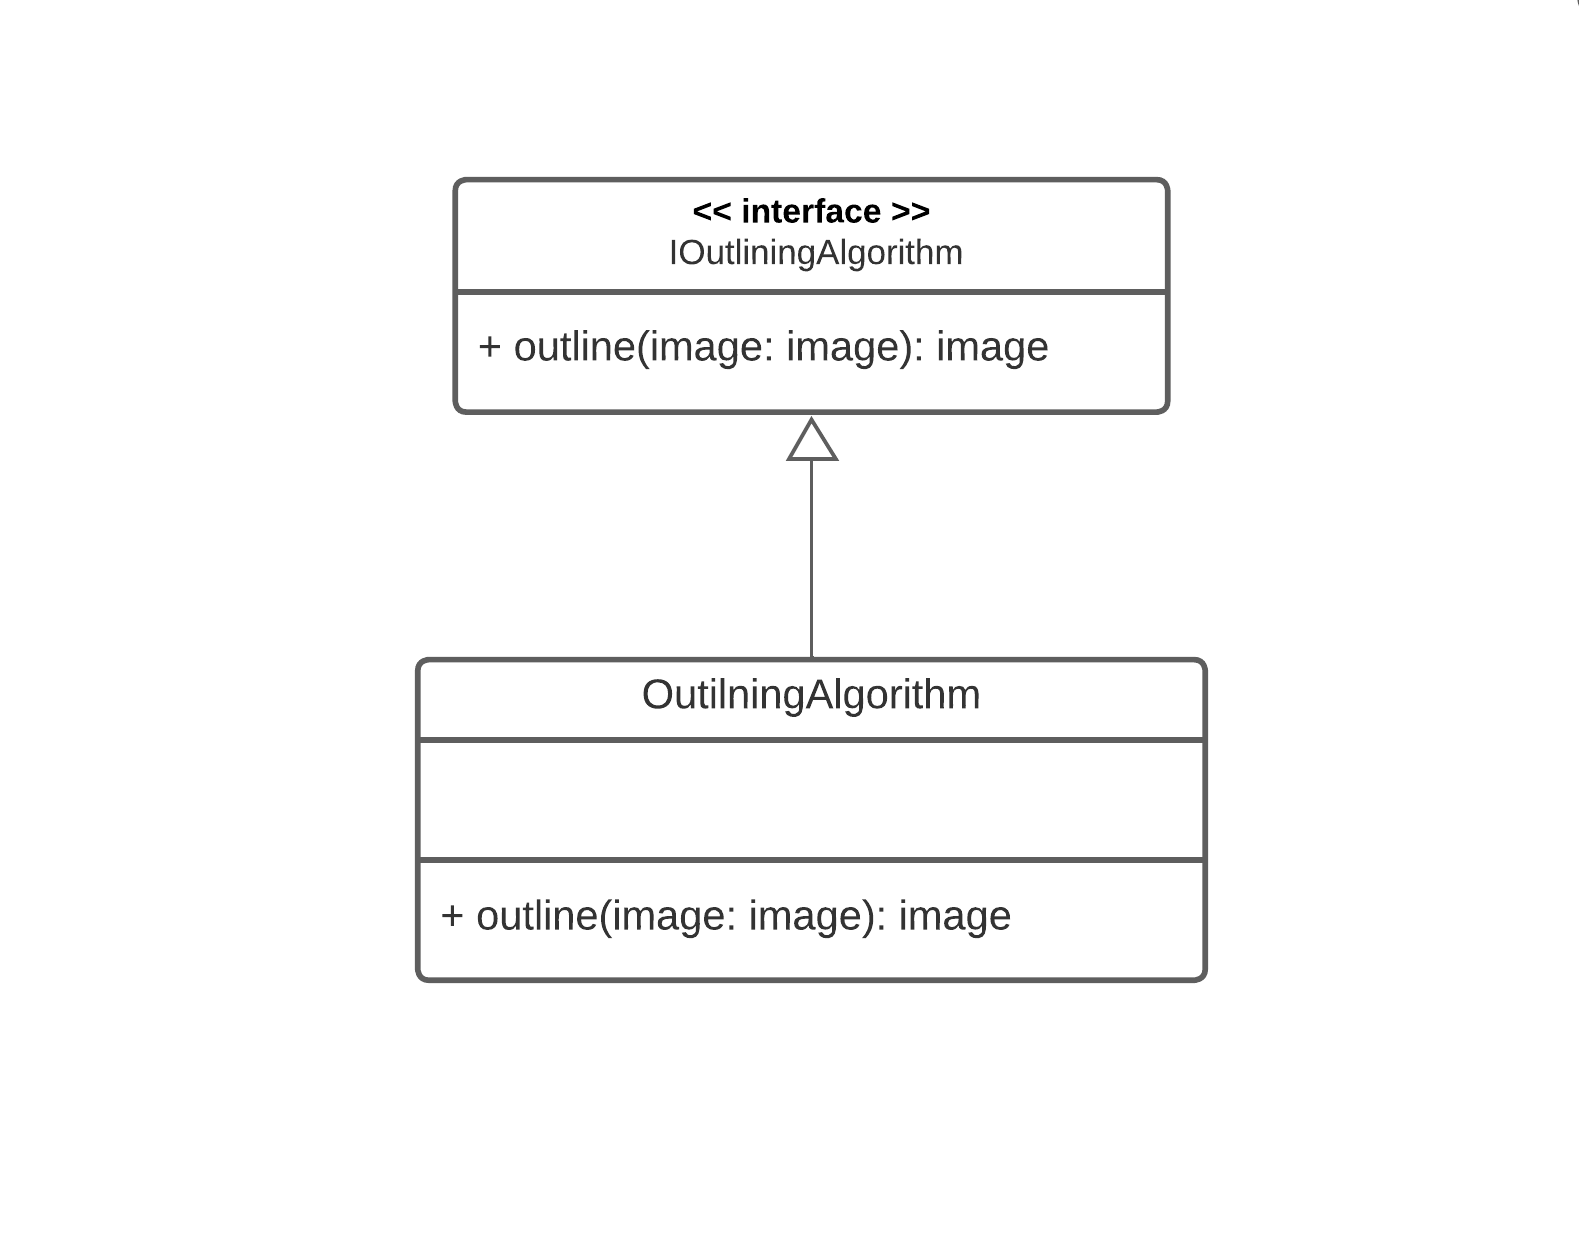
\includegraphics[scale = 1.0]{img/outlineStrategy.png}\\
    \caption{Strategy pattern dell'algoritmo di rielaborazione dell'immagine}
\end{figure}

Attualmente, la classe astratta "IOutliningAlgorithm" ha una sola classe concreta che rappresenta l'unico algoritmo implementato. Tuttavia, è progettata in modo da consentire l'estensione per l'implementazione di ulteriori 
algoritmi in futuro. Ciò significa che se si desidera aggiungere nuovi algoritmi, 
sarà possibile creare nuove classi che estendono l'interfaccia astratta "IOutliningAlgorithm". 
Questa flessibilità consente di espandere il sistema per includere più algoritmi di scontorno delle immagini senza dover 
modificare la struttura di base.

\begin{figure}[H]
    \centering
    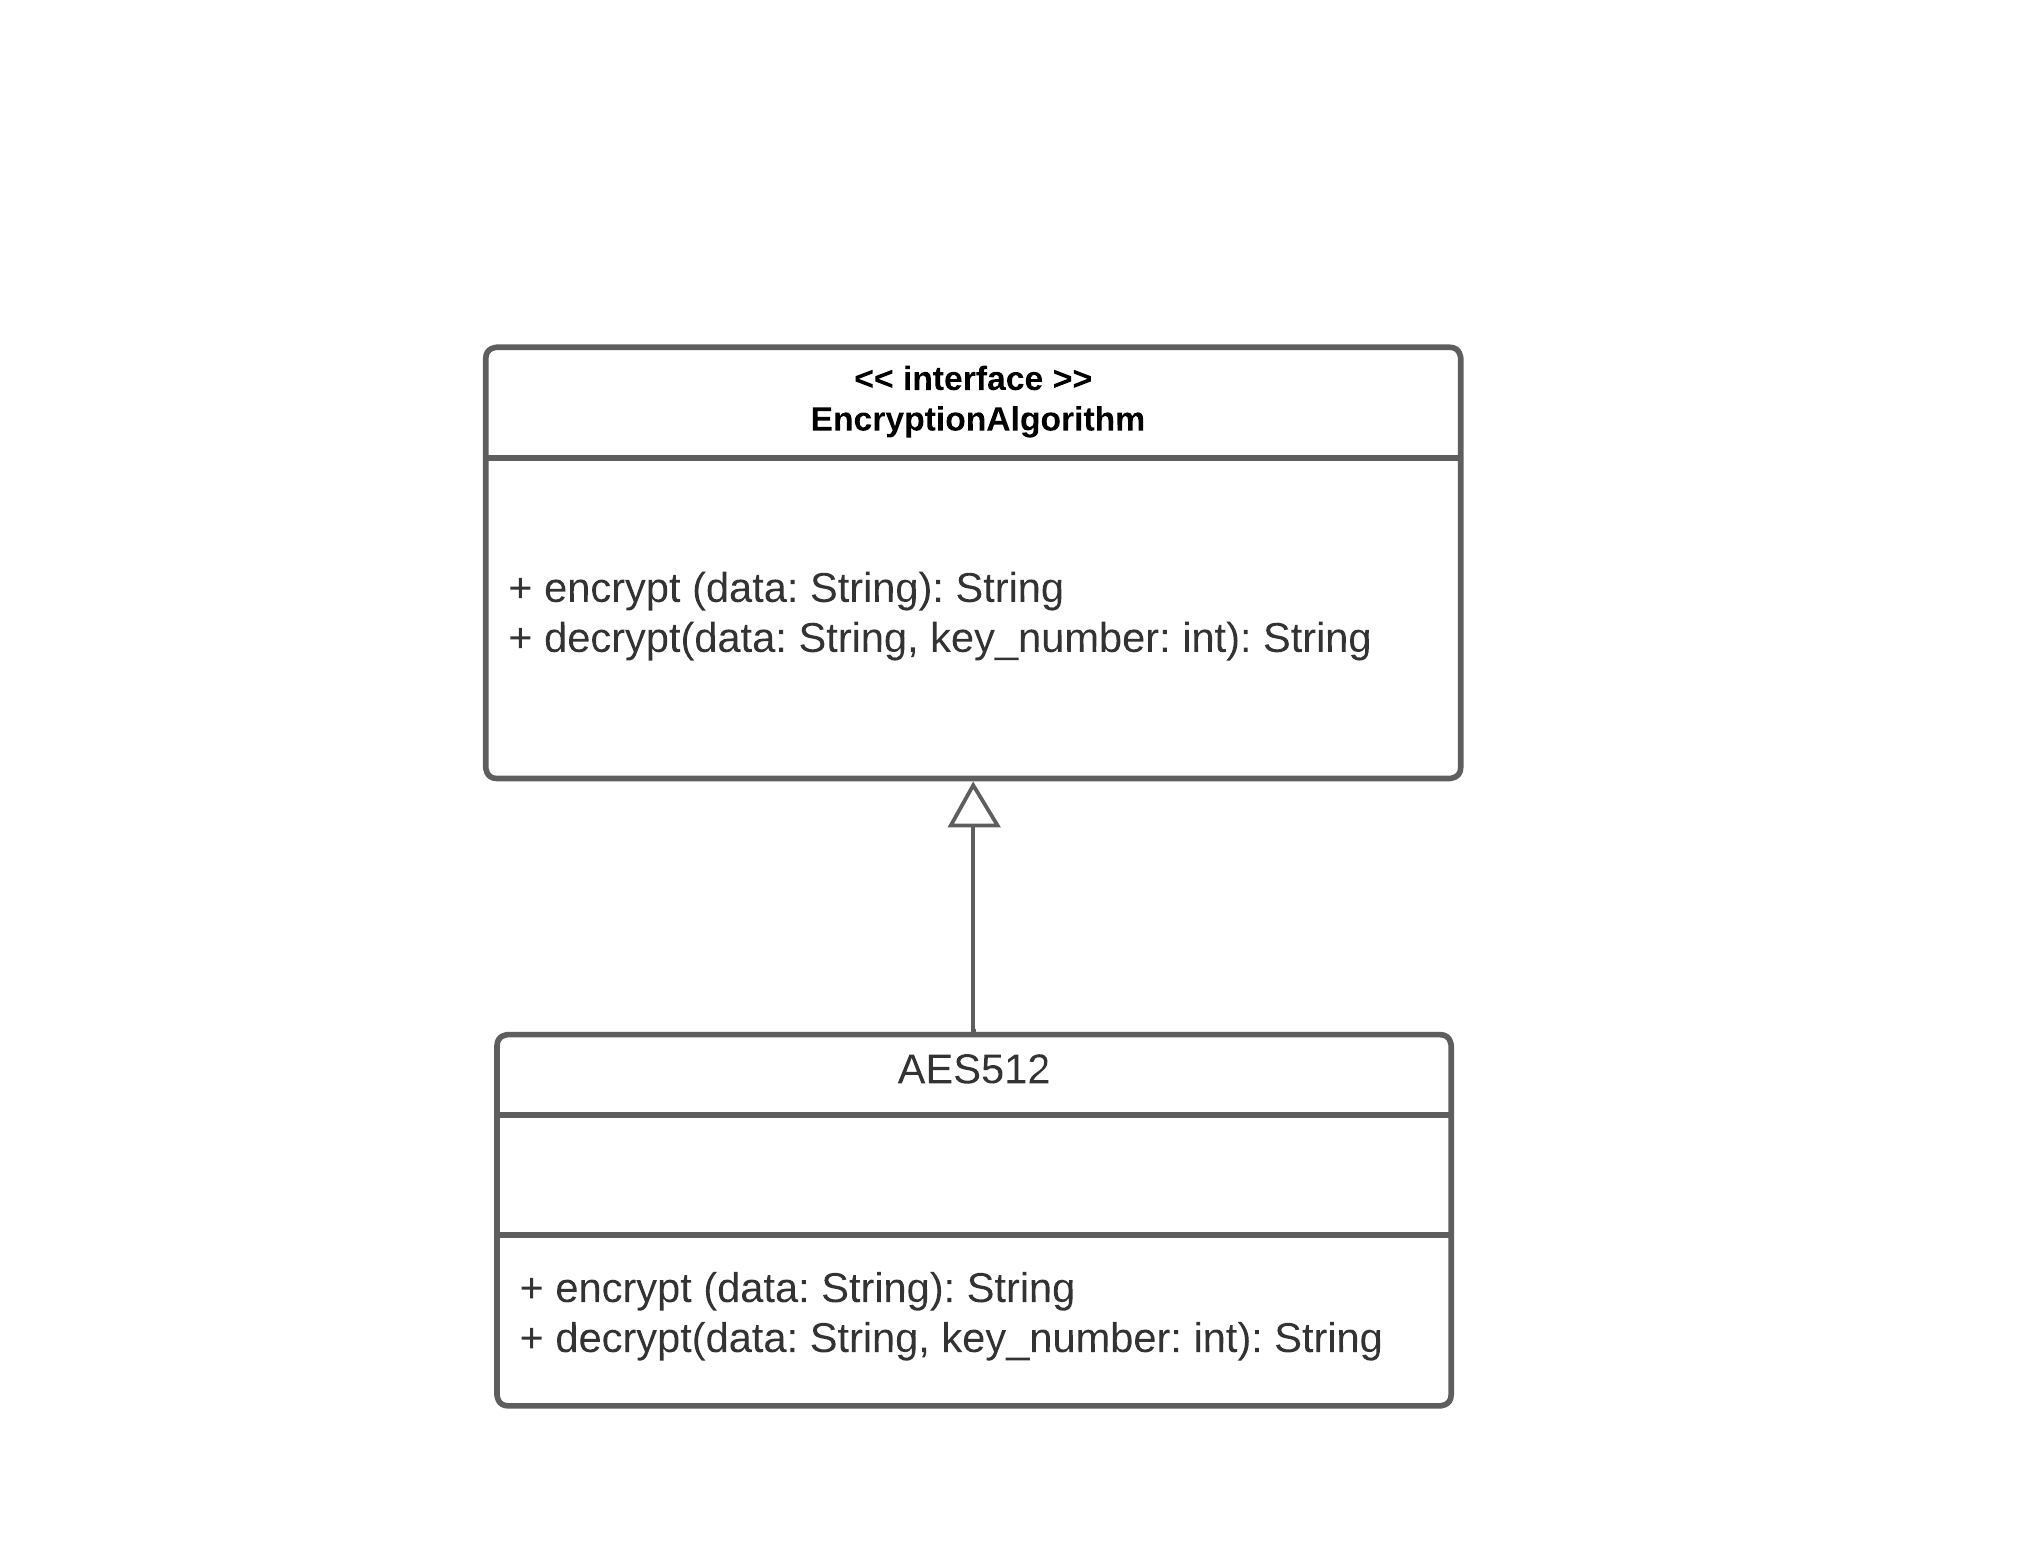
\includegraphics[scale = 1.0]{img/criptStrategy.png}\\
    \caption{Strategy patter dell'algoritmo per l'encrypting}
\end{figure}

Come sopra, la classe astratta "EncryptionAlgorithm" ha una sola classe concreta per il motivo sopra citata.

\subsubsection{Dependency Injection}

\begin{figure}[H]
    \centering
    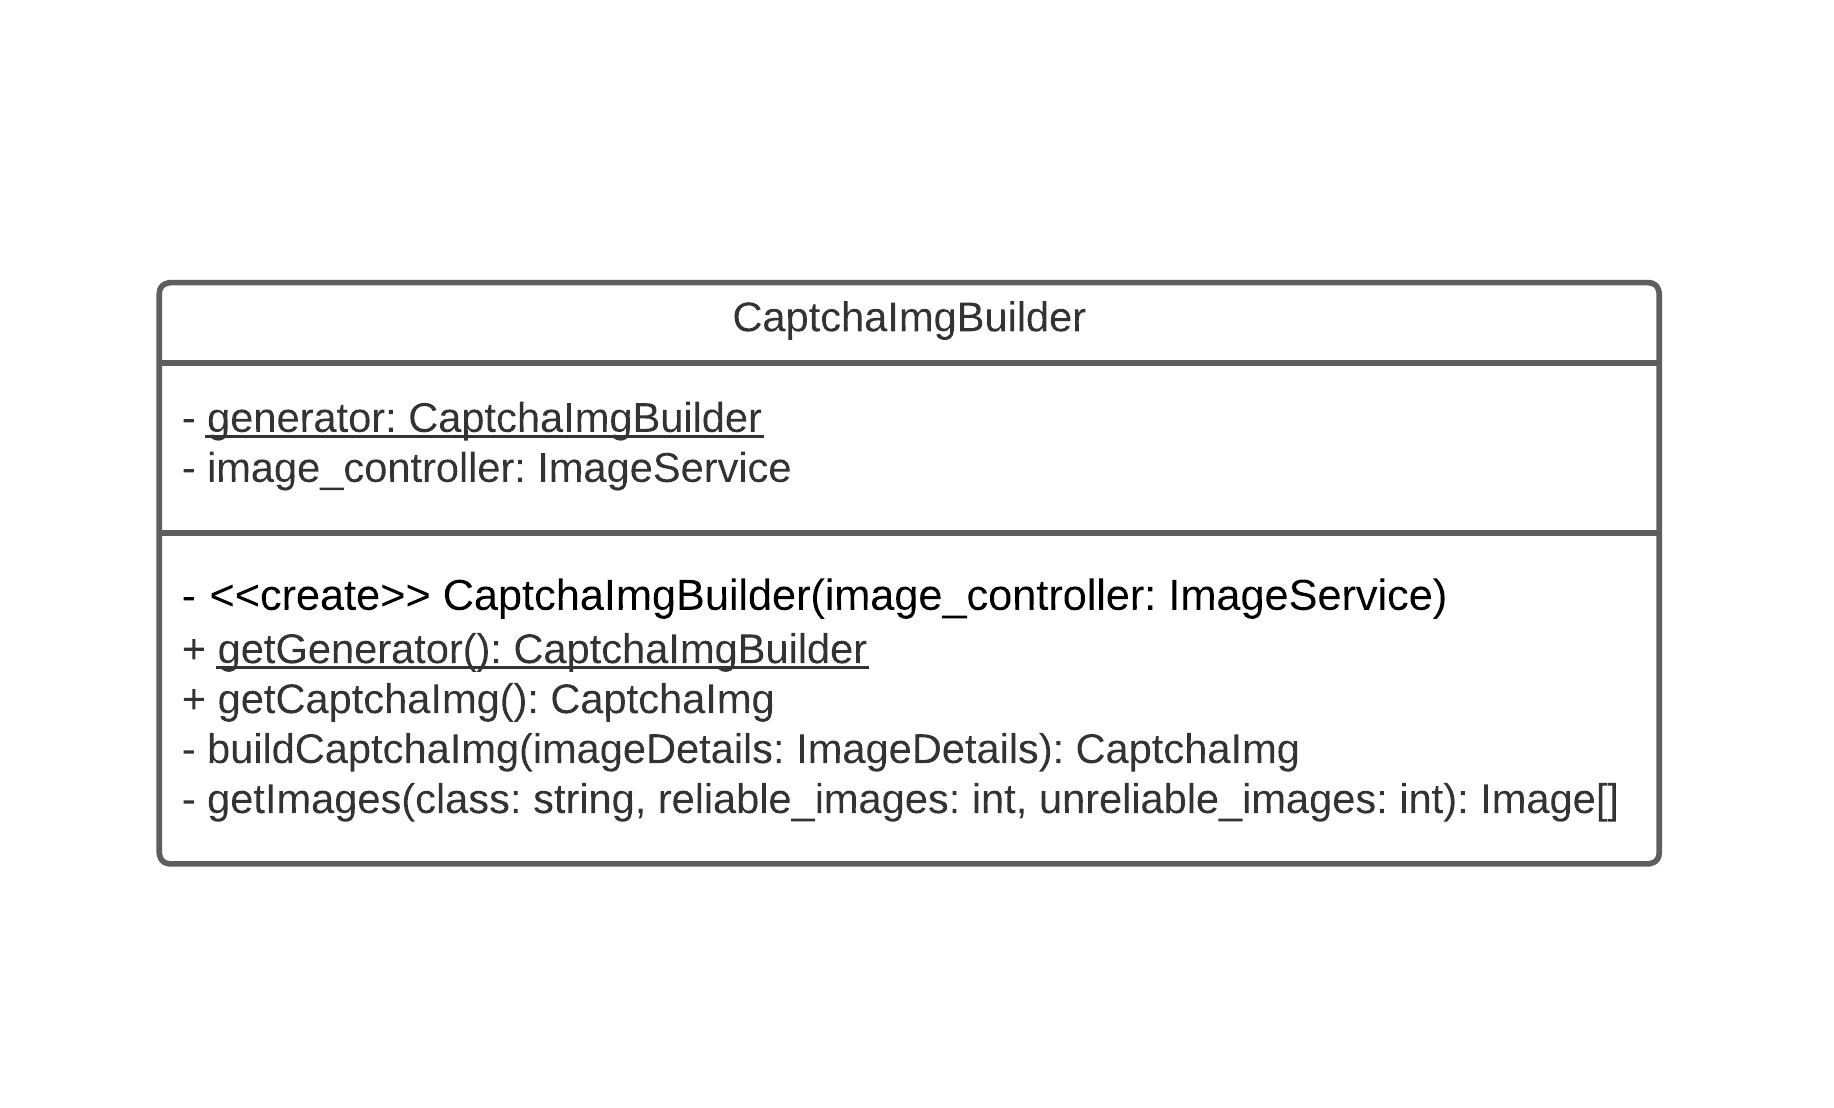
\includegraphics[scale = 1.0]{img/singleton.png}\\
    \caption{Singleton pattern}
\end{figure}

La costruzione di un'instanza di CaptchaImg è un'operazione che può essere considerata complessa in quanto
bisogna tenere in considerazione variabili come numero di classi di immagine presenti e numero di immagini per classe,
tali variabili devono a loro volta rispettare delle condizioni:
\begin{itemize}
    \item numero di classi tra 2 e 4 estremi compresi
    \item 9 immagini totali
    \item le immagini della classe target devono essere la metà + 1 affidabili
    \item le immagini delle classi non target devono essere la metà affidabili
\end{itemize}
Per quanto sopra si è deciso si spezzare la complessità e creare una classe il cui compito è quello di rifornire il costruttore
di CaptchaImg. 

\subsubsection{Strategy Pattern}

Il pattern Strategy è stato utilizzato per l'algoritmo di scontornamento delle immagini e per quello di cifratura.
L'utilizzo di tale pattern permette una futura estensione delle famiglie degli algoritmi in questione.


\subsubsection{Model-View-Controller}
Il pattern architetturale su cui si basa il framework Laravel è \textit{Model-View-Controller}.
Lo sviluppo del servizio API per la generazione e verifica del captcha sfrutta la classi messe a disposizione del framework:
\begin{itemize}
    \item Illuminate\\Database\\Eloquent\\Model: classe astratta per lo sviluppo di modelli la quale fornisce attributi e metodi integrati per la comunicazione con il database
    \item Illuminate\\Routing\\Controller: classe astratta per lo sviluppo di classi il cui compito è la gestione delle route e dei modelli
\end{itemize}
Le viste trattandosi di un API non sono state utilizzate.

Questo pattern inoltre è alla base dello sviluppo dell'applicazione web utilizzata per testare il servizio di Captcha.